% Options for packages loaded elsewhere
\PassOptionsToPackage{unicode}{hyperref}
\PassOptionsToPackage{hyphens}{url}
\PassOptionsToPackage{dvipsnames,svgnames,x11names}{xcolor}
%
\documentclass[
  12pt,
]{article}
\usepackage{amsmath,amssymb}
\usepackage{iftex}
\ifPDFTeX
  \usepackage[T1]{fontenc}
  \usepackage[utf8]{inputenc}
  \usepackage{textcomp} % provide euro and other symbols
\else % if luatex or xetex
  \usepackage{unicode-math} % this also loads fontspec
  \defaultfontfeatures{Scale=MatchLowercase}
  \defaultfontfeatures[\rmfamily]{Ligatures=TeX,Scale=1}
\fi
\usepackage{lmodern}
\ifPDFTeX\else
  % xetex/luatex font selection
    \setmainfont[]{Palatino}
    \setsansfont[]{Helvetica}
    \setmonofont[]{Menlo}
\fi
% Use upquote if available, for straight quotes in verbatim environments
\IfFileExists{upquote.sty}{\usepackage{upquote}}{}
\IfFileExists{microtype.sty}{% use microtype if available
  \usepackage[]{microtype}
  \UseMicrotypeSet[protrusion]{basicmath} % disable protrusion for tt fonts
}{}
\makeatletter
\@ifundefined{KOMAClassName}{% if non-KOMA class
  \IfFileExists{parskip.sty}{%
    \usepackage{parskip}
  }{% else
    \setlength{\parindent}{0pt}
    \setlength{\parskip}{6pt plus 2pt minus 1pt}}
}{% if KOMA class
  \KOMAoptions{parskip=half}}
\makeatother
\usepackage{xcolor}
\usepackage[margin = 1.2in]{geometry}
\usepackage{color}
\usepackage{fancyvrb}
\newcommand{\VerbBar}{|}
\newcommand{\VERB}{\Verb[commandchars=\\\{\}]}
\DefineVerbatimEnvironment{Highlighting}{Verbatim}{commandchars=\\\{\}}
% Add ',fontsize=\small' for more characters per line
\newenvironment{Shaded}{}{}
\newcommand{\AlertTok}[1]{\textcolor[rgb]{1.00,0.00,0.00}{\textbf{#1}}}
\newcommand{\AnnotationTok}[1]{\textcolor[rgb]{0.38,0.63,0.69}{\textbf{\textit{#1}}}}
\newcommand{\AttributeTok}[1]{\textcolor[rgb]{0.49,0.56,0.16}{#1}}
\newcommand{\BaseNTok}[1]{\textcolor[rgb]{0.25,0.63,0.44}{#1}}
\newcommand{\BuiltInTok}[1]{\textcolor[rgb]{0.00,0.50,0.00}{#1}}
\newcommand{\CharTok}[1]{\textcolor[rgb]{0.25,0.44,0.63}{#1}}
\newcommand{\CommentTok}[1]{\textcolor[rgb]{0.38,0.63,0.69}{\textit{#1}}}
\newcommand{\CommentVarTok}[1]{\textcolor[rgb]{0.38,0.63,0.69}{\textbf{\textit{#1}}}}
\newcommand{\ConstantTok}[1]{\textcolor[rgb]{0.53,0.00,0.00}{#1}}
\newcommand{\ControlFlowTok}[1]{\textcolor[rgb]{0.00,0.44,0.13}{\textbf{#1}}}
\newcommand{\DataTypeTok}[1]{\textcolor[rgb]{0.56,0.13,0.00}{#1}}
\newcommand{\DecValTok}[1]{\textcolor[rgb]{0.25,0.63,0.44}{#1}}
\newcommand{\DocumentationTok}[1]{\textcolor[rgb]{0.73,0.13,0.13}{\textit{#1}}}
\newcommand{\ErrorTok}[1]{\textcolor[rgb]{1.00,0.00,0.00}{\textbf{#1}}}
\newcommand{\ExtensionTok}[1]{#1}
\newcommand{\FloatTok}[1]{\textcolor[rgb]{0.25,0.63,0.44}{#1}}
\newcommand{\FunctionTok}[1]{\textcolor[rgb]{0.02,0.16,0.49}{#1}}
\newcommand{\ImportTok}[1]{\textcolor[rgb]{0.00,0.50,0.00}{\textbf{#1}}}
\newcommand{\InformationTok}[1]{\textcolor[rgb]{0.38,0.63,0.69}{\textbf{\textit{#1}}}}
\newcommand{\KeywordTok}[1]{\textcolor[rgb]{0.00,0.44,0.13}{\textbf{#1}}}
\newcommand{\NormalTok}[1]{#1}
\newcommand{\OperatorTok}[1]{\textcolor[rgb]{0.40,0.40,0.40}{#1}}
\newcommand{\OtherTok}[1]{\textcolor[rgb]{0.00,0.44,0.13}{#1}}
\newcommand{\PreprocessorTok}[1]{\textcolor[rgb]{0.74,0.48,0.00}{#1}}
\newcommand{\RegionMarkerTok}[1]{#1}
\newcommand{\SpecialCharTok}[1]{\textcolor[rgb]{0.25,0.44,0.63}{#1}}
\newcommand{\SpecialStringTok}[1]{\textcolor[rgb]{0.73,0.40,0.53}{#1}}
\newcommand{\StringTok}[1]{\textcolor[rgb]{0.25,0.44,0.63}{#1}}
\newcommand{\VariableTok}[1]{\textcolor[rgb]{0.10,0.09,0.49}{#1}}
\newcommand{\VerbatimStringTok}[1]{\textcolor[rgb]{0.25,0.44,0.63}{#1}}
\newcommand{\WarningTok}[1]{\textcolor[rgb]{0.38,0.63,0.69}{\textbf{\textit{#1}}}}
\usepackage{graphicx}
\makeatletter
\def\maxwidth{\ifdim\Gin@nat@width>\linewidth\linewidth\else\Gin@nat@width\fi}
\def\maxheight{\ifdim\Gin@nat@height>\textheight\textheight\else\Gin@nat@height\fi}
\makeatother
% Scale images if necessary, so that they will not overflow the page
% margins by default, and it is still possible to overwrite the defaults
% using explicit options in \includegraphics[width, height, ...]{}
\setkeys{Gin}{width=\maxwidth,height=\maxheight,keepaspectratio}
% Set default figure placement to htbp
\makeatletter
\def\fps@figure{htbp}
\makeatother
\setlength{\emergencystretch}{3em} % prevent overfull lines
\providecommand{\tightlist}{%
  \setlength{\itemsep}{0pt}\setlength{\parskip}{0pt}}
\setcounter{secnumdepth}{5}
\ifLuaTeX
\usepackage[bidi=basic]{babel}
\else
\usepackage[bidi=default]{babel}
\fi
\babelprovide[main,import]{french}
\ifPDFTeX
\else
\babelfont{rm}[]{Palatino}
\fi
% get rid of language-specific shorthands (see #6817):
\let\LanguageShortHands\languageshorthands
\def\languageshorthands#1{}
\ifLuaTeX
  \usepackage{selnolig}  % disable illegal ligatures
\fi
\usepackage{bookmark}
\IfFileExists{xurl.sty}{\usepackage{xurl}}{} % add URL line breaks if available
\urlstyle{same}
\hypersetup{
  pdftitle={OpenYourMind},
  pdfauthor={Dibassi Brahima, Samar Lahmar, Farouck Cherfi},
  pdflang={fr},
  colorlinks=true,
  linkcolor={Maroon},
  filecolor={Maroon},
  citecolor={Blue},
  urlcolor={NavyBlue},
  pdfcreator={LaTeX via pandoc}}

\title{OpenYourMind}
\usepackage{etoolbox}
\makeatletter
\providecommand{\subtitle}[1]{% add subtitle to \maketitle
  \apptocmd{\@title}{\par {\large #1 \par}}{}{}
}
\makeatother
\subtitle{Projet final : Moteur de recherche d'une bibliothèeque.}
\author{Dibassi Brahima, Samar Lahmar, Farouck Cherfi}
\date{03 Avril 2024}

\begin{document}
\maketitle

\newpage

{
\hypersetup{linkcolor=}
\setcounter{tocdepth}{3}
\tableofcontents
}
\newpage

\section{Introduction}\label{introduction}

Ce rapport présente le développement d'une application multisupport de
moteurs de recherche de documents dans une bibliothèque de livres au
format textuel. Une application multisupport se distingue d'une simple
page web par sa capacité à interagir avec l'utilisateur, offrant des
fonctionnalités dynamiques et réactives. Ce projet met l'accent sur deux
aspects essentiels : la pertinence et la performance du moteur de
recherche. La pertinence est évaluée à l'aide de tests utilisateurs,
tandis que la performance est mesurée à travers les temps de réponse du
moteur de recherche.

\section{Setup}\label{setup}

\subsection{Installation}\label{installation}

\subsubsection{Backend}\label{backend}

\begin{itemize}
\tightlist
\item
  Python \textgreater= 3.12

  \begin{itemize}
  \tightlist
  \item
    \href{https://www.djangoproject.com/}{Django}
  \item
    \href{https://www.nltk.org/}{Nltk}
  \item
    \href{https://networkx.org/}{Networkx}
  \item
    \href{https://docs.python-requests.org/en/master/}{Requests}
  \end{itemize}
\end{itemize}

\begin{Shaded}
\begin{Highlighting}[]
\ExtensionTok{pip}\NormalTok{ install django djangorestframework nltk requests networkx}
\end{Highlighting}
\end{Shaded}

\subsubsection{Construction de la base de
données}\label{construction-de-la-base-de-donnuxe9es}

La base de données n'est pas incluse dans le rendu. Vous devez la
construire vous-même, cela prend BEAUCOUP DE TEMPS ET DE RESSOURCES.

\begin{Shaded}
\begin{Highlighting}[]
\BuiltInTok{cd}\NormalTok{ backend}
\ExtensionTok{python}\NormalTok{ manage.py makemigrations}
\ExtensionTok{python}\NormalTok{ manage.py migrate}
\ExtensionTok{python}\NormalTok{ manage.py scrape\_books}
\ExtensionTok{python}\NormalTok{ manage.py create\_indexTable}
\ExtensionTok{python}\NormalTok{ manage.py create\_metadata}
\end{Highlighting}
\end{Shaded}

\subsubsection{Frontend}\label{frontend}

\begin{itemize}
\tightlist
\item
  \href{https://flutter.dev/}{Flutter}
\end{itemize}

Pour installer \href{https://flutter.dev/}{Flutter}, voir la
\href{https://flutter.dev/docs/get-started/install}{documentation
officielle}.

\newpage

\subsection{Démarrage}\label{duxe9marrage}

\subsubsection{Backend}\label{backend-1}

Pour démarrer le serveur, exécuter la commande suivante~:

\begin{Shaded}
\begin{Highlighting}[]
\BuiltInTok{cd}\NormalTok{ backend}
\ExtensionTok{python}\NormalTok{ manage.py runserver}
\end{Highlighting}
\end{Shaded}

\subsubsection{Frontend}\label{frontend-1}

Pour démarrer l'application frontend, exécuter la commande suivante~:

\begin{Shaded}
\begin{Highlighting}[]
\BuiltInTok{cd}\NormalTok{ frontend}
\ExtensionTok{flutter}\NormalTok{ pub get}
\ExtensionTok{flutter}\NormalTok{ run}
\end{Highlighting}
\end{Shaded}

Puis choisissez l'appareil sur lequel vous souhaitez exécuter
l'application.

\section{Backend}\label{backend-2}

\subsection{Architecture}\label{architecture}

Le back est basé sur le framework Django, qui est un framework web
Python de haut niveau qui encourage un développement rapide et une
conception propre et pragmatique.

Au vu de la taille du projet, nous avons opté pour une architecture
simple de type monolithique, car elle est plus facile à gérer et à
déployer. Cependant, nous avons pris soin de séparer les partis métiers
et les parties de gestion de la base de données.

\subsubsection{Base de données}\label{base-de-donnuxe9es}

\begin{itemize}
\tightlist
\item
  \texttt{backend/gutendex/}

  \begin{itemize}
  \tightlist
  \item
    \texttt{management/commands/} : Commandes personnalisées pour la
    gestion de la base de données.

    \begin{itemize}
    \tightlist
    \item
      \texttt{create\_indexTable.py} : Création de la table d'index
      inversé.
    \item
      \texttt{create\_metadata.py} : Création des métadonnées des
      livres, utilisées pour l'affichage des résultats de recherche, le
      filtrage et le tri.
    \item
      \texttt{scrape\_books.py} : Récupération des 1660 premiers à
      partir de l'API de \href{https://www.gutenberg.org/}{Gutenberg}.
    \end{itemize}
  \item
    \texttt{models.py} : Définition des modèles de données.
  \end{itemize}
\end{itemize}

\textbf{Scraping (Farouck Cherfi) : }

\newpage

Voici à titre indicatif, un diagramme de la base de données :

\begin{figure}
\centering
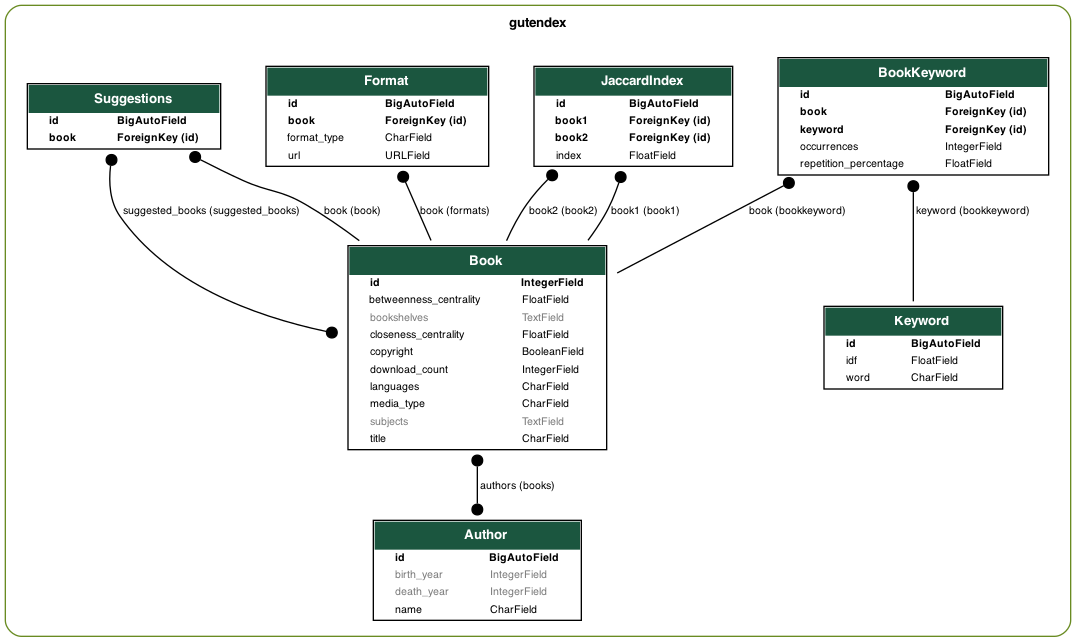
\includegraphics{../backend/db.png}
\caption{Database Diagram}
\end{figure}

\subsubsection{EndPoints}\label{endpoints}

\begin{itemize}
\tightlist
\item
  \texttt{top-books/} : Récupération des livres les plus téléchargés.
\item
  \texttt{search/\textless{}sentence\ or\ regex\textgreater{}/} :
  Recherche de livres par phrase.
\item
  \texttt{book/\textless{}bookid\textgreater{}/} : Récupération d'un
  livre par son identifiant.
\item
  \texttt{suggest/\textless{}bookid\textgreater{}/} : Suggestions de
  recherche.
\end{itemize}

\subsection{Recherche}\label{recherche}

\begin{itemize}
\tightlist
\item
  \texttt{backend/gutendex/helpers.py} : Fonctions de recherche.
\end{itemize}

Le moteur de recherche est basé sur l'indexation inversée des livres.
Une fois nos livres compatibles avec les mots clés récupérés, il est
important de les classer par pertinence.

\subsubsection{Heuristiques}\label{heuristiques}

Pour notre heuristique de classements, nous avons utilisé 3 valeurs :

\begin{itemize}
\tightlist
\item
  \textbf{AVERAGE TF-IDF} : Term Frequency-Inverse Document Frequency
  est une mesure statistique utilisée pour évaluer l'importance d'un mot
  dans un document par rapport à une collection de documents ici on
  utilise une version modifiée afin de prendre en compte un ensemble de
  mots clés.
\end{itemize}

Voici la formule utilisée pour calculer le TF d'un terme pour un
document:
\[TF(t) = \frac{\text{Nombre de fois où le terme apparaît dans le document}}{\text{Nombre total de termes dans le document}}\]
Voici la formule utilisée pour calculer l'IDF d'un terme:
\[IDF(t) = \log\left(\frac{\text{Nombre total de documents}}{\text{Nombre de documents contenant le terme}}\right)\]

\begin{itemize}
\item
  \textbf{Betweenness Centrality} : Elle mesure le nombre de fois qu'un
  nœud est sur le chemin le plus court entre deux autres nœuds.
\item
  \textbf{Closseness Centrality} : Elle mesure la distance moyenne entre
  un nœud et tous les autres nœuds.
\end{itemize}

Les deux dernières valeurs étant basées sur des graphes, voici sa
construction :

Soit \(G = (V, E)\) un graphe géométrique où \(V\) est l'ensemble des
livres et \(E\) l'ensemble des arêtes.

On construit \(E\) de la manière suivante :

\begin{itemize}
\tightlist
\item
  On determine la moyenne des similarités de Jaccard entre chaque livre
  \[ k = \frac{\sum{v,u \in V*V} \text{Jaccard}(u, v)}{|V|*|V|-1}\ u \neq v\]
\item
  Pour éviter de se connecter a trop de livres, on augemente \(k\) de
  30\%. \[ threashold = k + 0.3k\]
  \[ E = \{(u, v) \in V \times V \mid \text{Jaccard}(u, v) \geq threashold\}\]
\end{itemize}

Une fois ses valeurs calculées, on les combine pour obtenir un score de
pertinence d'un livre par rapport à un ensemble de mots clés

\[Score(Keywords, Book) = 0.7*\text{AVG-TF-IDF}(Keywords, Book)\]
\[ +\ 0.15*\text{Betweenness}(Book) + 0.15*\text{Closeness}(Book)\]

\newpage

\subsection{Suggestions}\label{suggestions}

Dans le but d'améliorer l'expérience utilisateur, nous avons implémenté
un système de suggestions de recherche. Ce système est basé sur la
recherche de livres similaires à celui sélectionné par l'utilisateur.

Nous avons utilisé essayer deux approches pour déterminer la similarité
entre les livres :

\subsubsection{Similarité par le
titre}\label{similarituxe9-par-le-titre}

Ici, l'approche est basée sur le titre du livre. La méthode est la
suivante :

\begin{enumerate}
\def\labelenumi{\arabic{enumi}.}
\tightlist
\item
  On récupère les mots clés du titre.
\item
  On relance une recherche avec les deux mots clés ayant le plus grand
  IDF.
\item
  On retourne les résultats.
\end{enumerate}

\subsubsection{Similarité par le
contenu}\label{similarituxe9-par-le-contenu}

Ici l'approche place plus d'emphase sur le contenu, La méthode est la
suivante, on récupère simplement les livres connectés sur le graphe
décrit \hyperref[heuristiques]{précédemment}.

\subsubsection{Comparaison}\label{comparaison}

Nous avons choisi après plusieurs tests d'éliminer la première méthode,
car dans les cas où le titre contient des mots très courants, la
recherche n'est pas pertinente. Un exemple de titre non pertinent est
``Le Rouge et le Noir'', les mots clés Rouge/Noir ne permettent pas de
déterminer des informations sur le contenu du livre et donc notre
\hyperref[heuristiques]{AVG-TF-IDF} n'est pas pertinent, invalidant la
méthode de scoring.

\subsection{Performance}\label{performance}

Dans cette section, nous allons discuter de la performance de notre
moteur de recherche. Nous avions un objectif principal :

\begin{itemize}
\tightlist
\item
  Réduire le temps de réponse du moteur de recherche
\end{itemize}

Pour ce faire, nous avons utilisé une technique principale le précalcul,
ainsi nous avons precalculé les valeurs de
\hyperref[heuristiques]{Betweenness},
\hyperref[heuristiques]{Closeness}, \hyperref[heuristiques]{TF-IDF} pour
chaque livre et chaque mot clé.

\subsubsection{Tests}\label{tests}

Nous avons testé la performance de notre moteur de recherche sur un
ensemble de 140 requêtes de type keyword/regex aléatoire. Voici les
résultats de nos tests :

\begin{figure}
\centering
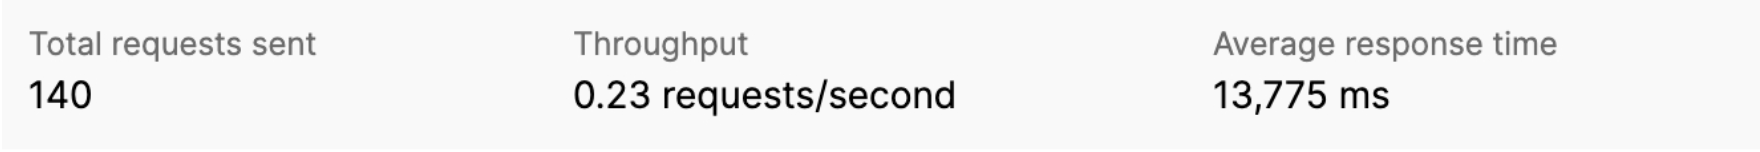
\includegraphics{./avgTotal.png}
\caption{Average Response Time}
\end{figure}

\begin{figure}
\centering
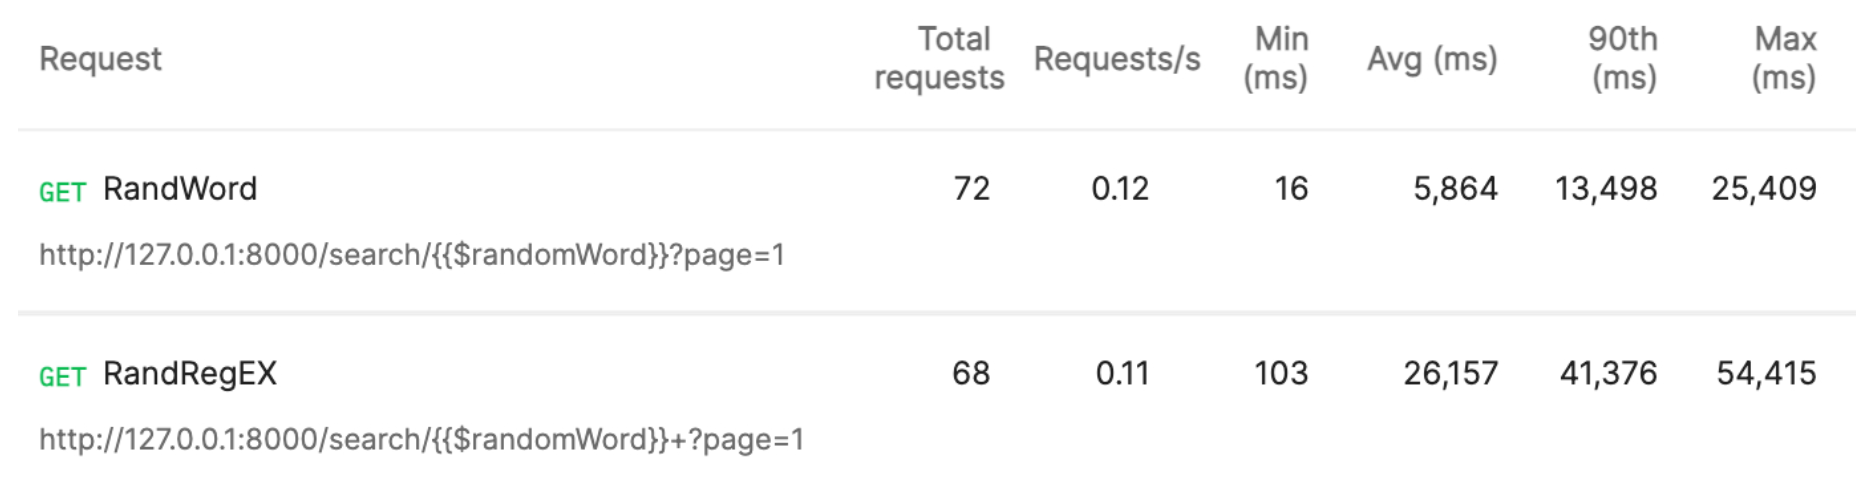
\includegraphics{./avgPerEndPoint.png}
\caption{Per Endpoint Response Time}
\end{figure}

\section{Frontend}\label{frontend-2}

\section{Conclusion}\label{conclusion}

\end{document}
